\documentclass[12pt]{book}
%% Packages élémentaires %%
\usepackage[utf8]{inputenc}
\usepackage{mathpazo,etoolbox, graphicx, wrapfig, pbox, fancybox, hyperref, appendix, geometry, amsmath, amssymb, tikz, pgfplots, calc, enumitem}
\graphicspath{{images/}}
\geometry{hmargin=2.4cm, vmargin = 2.1cm}
\setlist[itemize]{itemsep=10pt, label={--}}

%% Couleurs %%
\usepackage{xcolor}
\definecolor{bleu}{RGB}{14, 68, 175}
\definecolor{bleu3}{RGB}{222, 233, 255 }
\definecolor{orange2}{RGB}{255, 216, 154}
\definecolor{rouge}{RGB}{201, 0, 0}
\definecolor{vert}{RGB}{14, 137, 0}
\definecolor{gris}{RGB}{222,230,230}
\newcommand\rouge[1] {{\color{rouge}{#1}}}
\newcommand\bleu[1] {{\color{bleu}{#1}}}
\newcommand\green[1]{{\color{vert}{#1}}}


%% Cadres %%
\newcommand\bb[1]{
\begin{center}
\fcolorbox{black}{bleu3}{\parbox{\textwidth}{ 
#1
}}
\end{center}}

\newcommand\boite[1]{
\begin{center}
\fbox{\parbox{\textwidth}{ \begin{center}
\begin{Large}
#1
\end{Large}
\end{center}}}
\end{center}}

\newcommand\aparte[1]{
\begin{center}
\fcolorbox{white}{gris}{\parbox{\linewidth}{ \textit{A parte} \\
#1 }}
\end{center}}

\newcommand\exemple[1]{
\begin{center}
\fcolorbox{white}{gris}{\parbox{\linewidth}{ \textit{Exemple} \\
#1 }}
\end{center}}

%% Commandes %%
\newcommand\imp[1]{\underline{\textbf{#1}}}
\newcommand\eq[1]{\begin{large}
\begin{align*}
#1
\end{align*}
\end{large}}
%% Commandes fantaisistes (cf. Internet) %%
\renewcommand{\parallel}{ \mathbin{\!/\mkern-5mu/\!} }
\newcommand{\q}[1]{{%
\font\larm = larm1000%
\larm%
\char 190}{ \textit{#1} }{%
\font\larm = larm1000%
\larm%
\char 191}}

%% Wrapping %%
\newcommand\wrap[4]{\begin{wrapfigure}[#1]{#2}{#3\textwidth}
#4
\end{wrapfigure}}

\title{Synthèse du cours d'Électricité \\ \strut \\
\normalsize{\textit{Deuxième partie : théorie des champs}}}
\author{Sami \textsc{Abdul Sater}}

\begin{document}
\begin{titlepage} 


\begin{figure}[h]
\maketitle
    \begin{minipage}[c]{\textwidth}
        \centering
        \begin{center}
        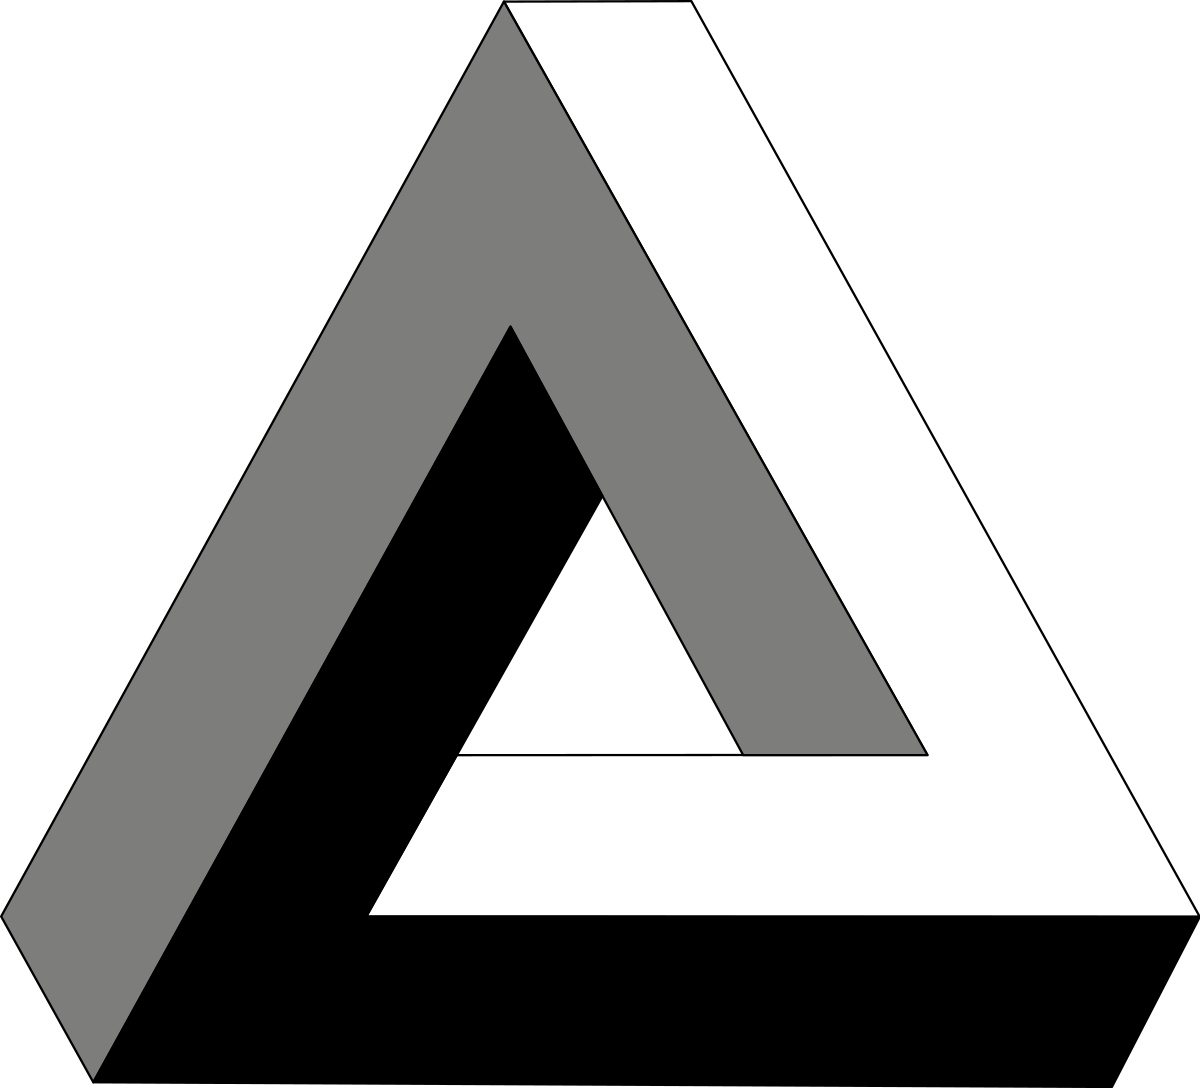
\includegraphics[scale = 0.13]{penrose.png}
        \end{center}
        
    \end{minipage}
\end{figure}
\end{titlepage}

\tableofcontents
\chapter{Introduction à la théorie des champs}
\section{Les équations de Maxwell}
Les équations de Maxwell permettent d'expliquer presque tous les phénomènes électromagnétiques, qui sont eux caractérisés par des forces qui apparaissent entre des objets. La \textbf{propriété fondamentale} qui explique ces phénomènes est la \textbf{charge électrique}. En pratique, c'est toujours la \textbf{force} qu'on observe. On déduit qu'elle est due à un champ, qui lui même est provoqué par la présence d'une charge. On considère en effet que les \textbf{charges électriques} sont des sources de champs électromagnétiques, par leur simple présence ou leur déplacement. Attention : une charge électrique ne provoque pas de force sur elle-même. Autrement dit :

\bo{Une charge n'est pas sensible à son propre champ.}
Le gang des phénomènes électromagnétiques se départagent en deux parties : ceux dus à la simple présence des charges électriques et ceux dus à leur déplacement. Il s'agit respectivement des phénomènes électriques et des phénomènes magnétiques.
\section{Champ ?}
Un champ est simplement une grandeur présente partout définie dans l'espace. Cela peut être un champ scalaire ou un champ vectoriel.
\section{Les outils de l'analyse vectorielle}
Petit rappel du cours de Physique Générale I et faisant écho au cours d'Analyse II, cette section reste néanmoins intéressante parce qu'elle se situe d'un point de vue différent ce ces cours. \\

La section présente donc des définitions de grandeurs d'analyse vectorielle : divergence, rotationnel, flux, etc.
\subsection{Flux}
Par définition, le flux d'un champ vectoriel $\vec{A}$ est l'intégrale de celui-ci sur une surface (celle sur laquelle on calcule le flux), en produit scalaire avec le vecteur normal de surface.

\eq{\phi = \iint_S \vec{A}.d\vec{S}}
Il s'agit d'une grandeur scalaire, d'une grandeur \textbf{macroscopique}. Un flux peut être interprété comme un débit. Par exemple : $$ I = \iint_S \vec{J}.d\vec{S}, $$ avec $\vec{J}$ le vecteur \textbf{densité de courant}. Une autre manière de l'interpréter est de se dire qu'il s'agit de la mesure de \textit{combien de champ $\vec{A}$ passe à travers le total de la surface}.
\subsection{Circulation}
La circulation d'un champ vectoriel $\vec{A}$ est l'intégrale du produit scalaire de ce champ par un vecteur de \q{chemin}, de longueur $L$ :

\eq{\zeta = \int_L \vec{A}.d\vec{l}}
On retrouve la définition du travail lorsque $\vec{A}$ est un champ de forces.
\subsection{Divergence}
La divergence d'un champ vectoriel $\vec{A}$ est un scalaire qui correspond à la valeur de flux de ce champ à travers une surface minuscule, divisé par cette surface. Ca c'est pour le rappel à PHYS-H1001. Mathématiquement, 

\eq{div(\vec{A}) = \sum_{i=1} ^n \dfrac{\partial A_i}{\partial x_i}}

Une divergence non nulle veut donc dire que le champ varie dans l'espace (divergence = disposition spatiale du champ vectoriel). Une divergence positive veut dire que c'est une quantité positive de champ $\vec{A}$ qui quitte l'élément en lequel on calcule la divergence. Cela veut dire que

 \eq{\div \vec{A} (x) > 0 \iff x \text{ est une source !}}
 Inversément, une divergence négative signifie que $x$ est un puits.

 \subsection{Rotationnel}
 La définition mathématique du rotationnel est :
 
 \eq{\rot \vec{A} = \left( \dfrac{\partial A_z}{\partial y} - \dfrac{\partial A_y}{\partial z} \right) \vec{1}_x +\left( \dfrac{\partial A_x}{\partial z} - \dfrac{\partial A_z}{\partial x} \right) \vec{1}_y +\left( \dfrac{\partial A_x}{\partial y} - \dfrac{\partial A_x}{\partial y} \right) \vec{1}_z }
 Physiquement, il représente un nouveau vecteur, $\rot \vec{A}$, qui a une orientation telle qu'un contour orienté dans cette direction permettra une circulation maximale. La norme correspond alors à cette circulation. Le rotationnel donne l'axe de rotation du champ vectoriel autour de lui même, autour du point de calcul.
 \subsection{Champs lamellaires et solénoïdaux}
 Tout champ vectoriel $\vec{A}$ peut être décomposé selon deux composantes : 
 \begin{enumerate}
 \item Une composante \textbf{lamellaire} ou \textbf{conservative}, $\vec{A}_{\text{lam}}$ dont le rotationnel est nul. Un champ lamellaire est représenté par des lignes de champ qui ne se croisent \textbf{jamais}.
 \item Une composante \textbf{solénoïdale} $\vec{A}_{\text{sol}}$ dont la divergence est nulle. Un champ solénoïdal est représenté par des lignes de champ circulaires.
 \item[$\Rightarrow$] $\vec{A} = \vec{A}_{\text{lam}} + \vec{a}_{\text{sol}}$
 \end{enumerate}
 
 \subsection{Gradient d'un champ scalaire}
 Un gradient d'un champ scalaire est un \textbf{champ vectoriel} qui représente l'accroissement maximal de la fonction, en norme et en direction. Alors, mathématiquement, on a :
 
 \eq{\grad( u) = \sum_{i=1} ^n \dfrac{\partial u}{\partial x_i} \vec{1}_{x_i}}
 On peut dès lors associer à toute variation de la fonction $u$ à ce gradient : $$du = \grad u \cdot  d\vec{l},$$ par exemple, représente l'accroissement de $u$ le long d'un élément de contour $d\vec{l}$. On se rend compte de cette simple écriture que la variation de $u$ entre deux points est donnée par l'intégrale du gradient. Finalement, si on effectue un contour fermé, on intègre d'un point à un même point et ça nous donne zéro. Donc la circulation du gradient de tout champ scalaire sur un contour fermé est \textbf{nulle}.
 \subsection{Potentiel scalaire d'un champ conservatif}
 Si un champ est conservatif, ça veut dire que son rotationnel est nul, et en vertu du théorème de Stokes, que sa circulation sur un contour fermé est nulle, tout comme le gradient d'un champ scalaire tient. Alors cela nous amène à définir un champ scalaire qu'on nomme \textbf{potentiel}, tel qu'en en prenant le gradient on tombe sur notre champ $\vec{A}$ à rotationnel nul. Grâce à la définition d'un champ scalaire qu'on note $U$ par exemple, on peut écrire la circulation de $\vec{A}$ très facilement :
 
 \equ{eq:gradient}{\int_a ^b \rouge{\vec{A}} \cdot d\vec{l} = \int_a ^b \rouge{\grad U} \cdot d\vec{l} = U(b)  - U(a)}
 On peut donc associer un potentiel scalaire à tout champ conservatif, et celui-ci est, de plus, défini à une constante près (parce que si on prend $U' = U + v$ avec $v = C^{\text{ste}}$, la constante s'annule dans la variation de $U$, cf. équation \textbf{\ref{eq:gradient}}).
 
 \subsection{Laplacien}
 Le laplacien d'un champ \textbf{scalaire} est un opérateur qui nous renvoie un scalaire à partir d'un champ vectoriel. Il s'agit de la divergence de son champ gradient :
 
 \eq{\Delta A = \div \left(\grad A \right))}
 On peut prendre le laplacien d'un champ \textbf{vectoriel} aussi, il s'agit de la somme des dérivées doubles, donc le produit de $\nabla^2$ par le champ vectoriel.
 
 \eq{\Delta \vec{A} = \nabla^2 \vec{A}}
 
 \section{Que signifient les équations de Maxwell ?}
  
  \begin{wrapfigure}[8]{r}{0.6\textwidth} 
  \vspace{-1cm}\maxwell
  \end{wrapfigure}
 Avec ce petit bagage mathématique que constituent les outils d'analyse vectorielle, on peut interpréter les équations de Maxwell. On voit qu'elles font intervenir les circulations et flux des champs $\vec{E}$ et $\vec{B}$, elles nous donnent donc une information quant aux composantes lamellaires et solénoïdales de ces champs. \\
 \begin{enumerate}
 \item La loi de Gauss donne la source de la composante lamellaire du champ électrique : c'est la présence d'une charge électrique $Q$. Le champ électrique converge ou diverge donc à un endroit (divergence non nulle car flux non nul).
 \item La loi de Faraday concerne la circulation de $\vec{E}$, donc le rotationnel de $\vec{E}$ et indique que la source de boucles de champ électrique est simplement la variation temporelle de champ magnétique.
 \item Il n'y a pas de monopole magnétique, donc la divergence (et donc le flux sur une surface fermée) de $\vec{B}$ est nulle.
 \item La loi d'Ampère formule que le champ magnétique $\vec{B}$ est purement \textbf{rotationnel}, et qu'il a 2 sources : les courants électriques $I$ et les variations de champ électrique. Tout comme la loi de Faraday indique pour le champ électrique, \textbf{$\vec{B}$ forme des boucles là où $\vec{E}$ varie dans le temps}.
 \end{enumerate}
 \section{Équation de continuité}
 On se souvient des sages paroles du sage sage Haelterman : cette équation porte pour de raisons obscures, le nom d'équation de continuité... \\
 
Il s'agit là du principe de conservation de la charge électrique, et elle peut être déduite des équations de Maxwell. En effet, en prenant la divergence de part et d'autre dans la loi d'Ampère forme locale 
\begin{eqnarray*}
\rot \vec{B} &=& \mu_0 \vec{J} + \varepsilon_0 \mu_0 \dfrac{\partial \vec{E}}{\partial t} \\
& \Leftrightarrow & \div \vec{J} = -\varepsilon_0 \dfrac{d}{dt} \div \vec{E} \\
&\Leftrightarrow & \div \vec{J} = -\dfrac{ \rho}{dt} \\
&\Rightarrow & \oint_S \vec{J} \cdot d\vec{S} = -\dfrac{dQ}{dt}
\end{eqnarray*}
\subsection*{Cas stationnaire}
Dans le cas stationnaire, les charges sont fixes et les courants sont constants, on a donc une intégrale de flux nulle sur $\vec{J}$, sa divergence est donc null, donc \textbf{$\vec{J}$ est, dans un cas de stationnarité, purement rotationnel}.
\chapter{Électrostatique dans le vide}
\section{Équations de Maxwell en statique}
\begin{wrapfigure}[8]{r}{0.3\textwidth} 
  \vspace{-1cm} \Large \maxwellvide
  \end{wrapfigure}
Les champs de ne varient pas dans le temps : les sources $\varrho$ et $\vec{J}$ sont constants dans le temps. Les équations de Maxwell prennent alors l'allure ci-contre. Par ailleurs, l'équation de continuité devient $\oint \vec{J}\cdot d\vec{S} = 0$.
\section{Champ électrique}
[Les formules sont connues et reprises à la fin de la section] \\ \\
On démontre la valeur du champ électrique généré par une charge $q_1$, à une distance $R$ de celle-ci par la loi de Gauss (avec une sphère entourant la charge, $A = 4\pi R^2$). On peut également généraliser à toute distribution de charge continue en remplaçant la charge simple $q_1$ par une intégrale la densité de charge volumique $\varrho$.
\section{Potentiel électrique}
Comme le champ électrique est purement lamellaire, on peut lui associer un champ scalaire qu'on nomme \q{potentiel électrique} $V$ tel que :

\eq{\vec{E} = - \grad (V) \Rightarrow V(B) - V(A)= \int_A ^B \grad(V) . d\vec{l} = -\int_A ^B \vec{E}.d\vec{l}}

On remarque que le gradient du potentiel et le champ électrique sont de sens opposé. Par ailleurs, le potentiel électrique est défini à une constante près, donc ce qu'on mesure c'est $V_{AB} = V(B)-V(A)$. Il s'agit de l'opposé du travail par unité de charge,

\eq{w_{AB} = \int_A ^B \vec{E}.d\vec{l},}
qui ne dépend pas du chemin suivi.
\subsection{Potentiel dû à une charge, à une distribution de charge}
On procède par intégration du champ électrique, en n'oubliant pas de prendre l'opposé. Finalement, pour l'électrostatique, on a :

\begin{eqnarray*}
\vec{E}_1 (P) &=& \dfrac{q_1}{4\pi \varepsilon_0 R^2} \vec{1}_R \\
\vec{E} (P) &=& \dfrac{1}{4\pi \varepsilon_0} \int_\tau
\dfrac{\varrho}{R^2} \vec{1}_R \\
V(P) &=& \dfrac{1}{4\pi \varepsilon_0} \dfrac{q}{R} \\
V(P) &=& \dfrac{1}{4\pi \varepsilon_0} \int_tau \dfrac{\varrho}{R} d\tau
\end{eqnarray*}
\subsection{Équation de Poisson}
L'équation de Poisson (obtenue en appliquant Gauss locale en exprimant le champ en fonction du potentiel) consiste en la déduction du potentiel à partir de la connaissance de la charge totale, ou la déduction de la distribution de charges à partir du potentiel. C'est une équation aux dérivées partielles qui nécessite des conditions aux limites pour être résolue ! Mais l'avantage c'est que la solution trouvée est unique.

\eq{\Delta V = \dfrac{\varrho}{\varepsilon_0}}
Sinon, dans le cas le plus général, \textbf{quand on connaît $\varrho(x,y,z)$}, soit on applique Gauss (symétrie) pour trouver $\vec{E}$, soit on calcule $V$ et prendre le gradient pour trouver $\vec{E}$.
\section{Énergie électrostatique}
\subsection{Cas d'une charge}
La définition de l'énergie électrostatique est le travail nécessaire pour ajouter une nouvelle charge dans le problème, c'est-à-dire amener une nouvelle charge $q_1$ là où il règne déjà un champ $\vec{E}$. On sait qu'il y aura une force répulsive à combattre, donc le travail à appliquer est $W = int -q_1\vec{E}.d\vec{l}$. Or, si on suppose que la charge vient de l'infini, on tombe sur :

\eq{W_e =  q_1 V(B)}
\subsection{Ensemble de charges}
La démonstration est effectuée progressivement, et reprise à la page 37-38.
\eq{W_e = \dfrac{1}{2} \int_\tau \varrho V d \tau}
\subsection{Densité d'énergie électrostatique}
Il s'agit de l'élément qu'on doit intégrer sur un volume $V$ pour obtenir l'énergie électrostatique $W_e$ obtenue au paragraphe précédent.

\eq{w_e = \dfrac{1}{2} \varepsilon_0 E^2}
\section{Conditions aux limites}
\subsection{Variation de champ $\vec{E}$}
Les \q{conditions aux limites} sont les équations supplémentaires qui expliquent le comportement, les relations de part et d'autre d'une surface chargée. Cela se fait à l'aide des deux équations de Maxwell concernant $\vec{E}$. En effet, on sait décomposer $\vec{E}$ en deux composantes : une tangentielle et une normale. On veut regarder la différence entre ces composantes de part et d'autre de la surface. 
\subsubsection{Composante normale}
On considère une surface chargée d'une densité $\varsigma$.
On applique Gauss sur un cylindre de hauteur infinitésimale et on obtient $E_{1n} - E_{2n} = \dfrac{\varsigma}{\varepsilon_0}$, soit une \textbf{discontinuité}.

\eq{\Vert \vec{E} \Vert \cdot \vec{1}_n = \dfrac{\varsigma}{\varepsilon_0}}
\subsubsection{Composante tangentielle}
On effectue l'intégrale de circulation sur un contour fermé et on obtient une continuité !

\bb{Au passage d'une surface chargée:
\begin{itemize}
\item La composante normale du champ électrique subit une discontinuité proportionnelle à la densité surfacique de charge
\item La composante tangentielle est continue.
\end{itemize}  }
\subsection{Variation de $V$}
La variation du potentiel s'étudie aussi selon sa dérivée normale. Concernant $V$, on peut effectuer l'intégrale de circulation de $\vec{E}$ sur un segment infinitésimal, mais alors cette intégrale est nulle, on a donc $V(2)-V(1) = -\int \vec{E}.d\vec{l} = 0 \iff V(2) = V(1)$. \\

Une autre manière d'étudier la variation de $V$ est de reprendre la discontinuité de $E_n$ et remplacer $E$ par $-\grad V$, donc $E_n$ par $\partial V / \partial n$. On obtient alors discontinuité de la dérivée normale du potentiel (proportionnelle à la densité surfacique de charge).

\bb{Potentiel :
\begin{itemize}
\item $V$ continu
\item Dérivée normale discontinue
\end{itemize}}
\section{Condensateurs et coefficient de capacité}
Le coefficient de capacité est la quantité de charges qu'emmagasine un condensateur par unité de potentiel. En pratique, avec $S$ la surface qui englobe une armature, et $L$ la distance entre les deux armatures :

\eq{C = \dfrac{Q}{V} = \dfrac{\oint_S \varepsilon_0 \vec{E}\cdot s\vec{S}}{-\int_L \vec{E} \cdot d\vec{l}}}
Pour un condensateur plan, on connaît la valeur du champ entre les deux plaques : il s'agit de deux fois le champ généré par une plaque infinie. Par Gauss, celui-ci vaut $E = Q/(2\varepsilon_0.A) \times 2 = \varsigma/ \varepsilon_0$. Si on écrit $Q$ comme $\varsigma  \cdot A$, on obtient

\bb{Condensateur plan : $C = \dfrac{\varepsilon_0 A}{d}$}
L'énergie accumulée par un condensateur est le travail qui a été nécessaire pour placer les charges $-Q$ et $+Q$ sur les armatures ! Il s'agit d'intégrer $\delta W = \delta q V = \delta q \dfrac{q}{C}$.

\bb{Énergie accumulée par un condensateur : $W_e = \frac{Q^2}{2C}$}
On peut également le montrer en intégrant la densité d'énergie magnétique vu qu'on connait le champ.
\section{Forces électrostatiques}
On peut calculer les forces présentes entre les armatures, principalement par bilan d'énergie. En effet, appliquer une force $F$ sur une distance $\delta d$ (dans le même sens) requiert un travail $\delta W = F \delta d$. La variation d'énergie engendrée par cette force doit être égale à la variation d'énergie du condensateur !

\eq{F_{ext} = \dfrac{\delta W}{\delta d} \qquad \text{où } \delta W = \delta \left( \dfrac{Q^2}{2C} \right) }
Alors soit on considère $C$ constant, dans quel cas il vaut $\varepsilon_0 A/d$ et on dérive $\delta W$ par rapport à $d$, soit on considère la ddp constante, mais on arrive à la force suivante :

\eq{F_{ext} = \dfrac{Q^2}{2\varepsilon_0 A}}
\section{Dipôle électrique}
Un dipôle électrique est un couple de 2 charges opposées, et séparées d'une distance $d$. On le caractérise par son \textbf{moment dipolaire} ($\vec{p} = q\vec{d}$ de la charge $-$ à la charge $+$), à partir duquel on peut calculer le potentiel généré. Le moment de forces agissant sur un dipôle, lui, est le produit vectoriel du moment dipolaire avec le champ électrique.

\eq{V(\vec{R}) = \dfrac{1}{4\pi \varepsilon_0} \dfrac{\vec{p} \cdot \vec{1}_R}{R^2} \qquad \vec{\tau} = \vec{p} \times \vec{E}}
\chapter{Milieux diélectriques}
\section{Étendre les équations de Maxwell aux milieux diélectriques}
\bfe{7}{0.3}{\vspace{-1cm} \begin{eqnarray*}
\div \vec{E}_p &=& \dfrac{\varrho_p}{\varepsilon_0} \\
\div \vec{E}_l &=& \dfrac{\varrho_l}{\varepsilon_0} \\
\vec{E} &=& \vec{E}_l + \vec{E}_p \\
\varrho &=& \varrho_l + \varrho_p \\
\end{eqnarray*}}
On avait défini le champ électrique $\vec{E}$ comme la force qu'on relevait expérimentalement, par unité de charge. On remarque maintenant qu'en présence d'un matériau diélectrique, on ne peut pas utiliser $\vec{E}$ tel qu'on le connait pour que la force soit entièrement décrite par ce-dernier.  Le champ qu'on connaît est généré par les charges sources du problèmes, on les appelle \textbf{charges libres} ($\varrho_l$). Alors ce qu'on fait, on \textit{suppose l'existence d'autres charges  ($\varrho_p$) qui provoquent un autre champ}.  Toutes ces charges répondent aux équations de Maxwell.  De cette manière, on peut toujours appliquer la loi de Gauss en prenant en compte les charges qui viennent d'autre part, les \textbf{charges de polarisation}.
\section{Matériaux diélectriques et polarisation}
\subsection{Hypothèses}
On stipule qu'un champ électrique dans un diélectrique provoque de nombreux dipôles de moments dipolaires $\vec{p}$. Ensemble, ils créent un champ électrique $\vec{E}_p$ qui s'additionne au champ $\vec{E}_l$ pour expliquer la force relevée. On quantifie les dipôles créés par leur \textbf{densité}. La \textbf{densité volumique de moment} est le \textbf{champ de vecteurs "Polarisation"} $\vec{P}$ tel que :

\begin{center}
$\vec{p} = \int_V \vec{P} dV \Rightarrow \left\{ \begin{array}{l}
\varrho_P = -\div \vec{P} \\
\varsigma_P = \vec{P} \cdot \vec{1}_n
\end{array} \right.$
\end{center}

Grâce à cela, on peut ré-exprimer le potentiel selon l'équation suivante :

\eq{V_P = \dfrac{1}{4\pi \varepsilon_0} \int_\tau \dfrac{\varrho_P}{R} d\tau + \dfrac{1}{4\pi \varepsilon_0} \oint_S \dfrac{\varsigma_P}{R} d\vec{S}}


\section{Champ de déplacement $\vec{D}$}
Grâce au fait d'exprimer $\sigma_P$ comme une divergence d'un champ, le champ polarisation, permet de s'amuser dans la loi de Gauss $\div \vec{E} = (\varrho_l + \varrho_P)/\varepsilon_0$, de sorte à faire apparaître que la densité de charges libres est la divergence d'un champ. On appelle ce nouveau champ ($\varepsilon_0 \vec{E} + \vec{P}$) le champ "Déplacement", noté $\vec{D}$.

\bb{$\vec{D} = \varepsilon_0 \vec{E} + \vec{P} \Rightarrow \div \vec{D} = \varrho_l$}
Pour conclure, on voit que prendre l'intégrale de flux de $\vec{D}$ sur une surface fermée nous donne la densité de charges libres renfermées par cette surface.
\section{Diélectriques linéaires}
On définit la \textit{permittivité} comme le lien entre $\vec{D}$ et $\vec{E}$. S'il est constant, on a un diélectrique linéaire. Mais pour que les deux champs soient proportionnels, il faut que $\vec{P} \propto \vec{E}$. On note ici le coefficient de proportionnalité $\chi_e$.

\eq{\vec{P} = \chi_e \varepsilon_0 \vec{E} \qquad \Rightarrow  \qquad \vec{D} = \varepsilon_0 (\bleu{1 + \chi_e}) \vec{E} \iff \bleu{\varepsilon_r = 1 + \chi_e}}

Un diélectrique est dit \textit{homogène} si la densité de charge de polarisation est proportionnelle à la densité de charges libres. On démontre que $\varrho_P = -\chi_e / \varepsilon_r \varrho_l$ (page 78).

\section{Interprétation des charges de polarisation}
Ne t'inquiètes pas ça va bien s'passer, bien s'passer ne t'inquiètes pas.
\section{Conditions aux limites}
Concernant le champ électrique total $\vec{E}$, on peut utiliser ce qu'on a déjà démontré : discontinuité de la composante normale proportionnelle à la densité surfacique de charge, et continuité de la composante tangentielle. Il faudra juste ajouter les densités de charges surfaciques de \textbf{polarisation} ! \\

Concernant le champ $\vec{D}$, lui on peut le traiter comme on avait fait avec $\vec{E}$ parce qu'il n'est produit que par des charges libres. On a donc discontinuité de la composante normale proportionnelle (\textbf{égale}) à la densité surfacique de charges libres. Quand la densité de charges libres est nulle, alors la composante normale de $\vec{D}$ est continue !

\eq{\Vert \vec{D} \Vert \cdot \vec{1}_n = \varsigma_l}

\bfe{3}{0.3}{\vspace{-1cm} \begin{eqnarray*}
\varepsilon_1 E_{1n} &=& \varepsilon_1 E_{1n} \\
E_{1t} &=& E_{2t}
\end{eqnarray*}}
Dans le cas où les deux régions sont des diélectriques de permittivités $\varepsilon_{1,2}$, on connaît la relation qui lie $\vec{D}_i$ à $\vec{E}_i$ : $\vec{D}_i = \varepsilon_i\vec{E}_i$. Quand il n'y a pas de charges libres à l'interface : $D_n$ continu, mais à cause de la relation présentée, les $E_n$ ne sont pas égaux, il n'y a pas de continuité de la composante normale.

\section{Condensateur plan avec diélectrique}
\subsection{Calcul du champ}
Deux contributions au champ : $\varsigma_l$, et $\varsigma_{\text{pol}} = \vec{P}\cdot \vec{1}_n$ (qu'on notera $P$). Comme on peut écrire, pour un linéaire, $P = \chi_e \varepsilon_0E$, on peut calculer le champ total en fonction de $\varsigma_l$ :

\eq{E = \dfrac{\varsigma_l - P}{\varepsilon_0} = \dfrac{\varsigma_l}{\varepsilon}}
\subsection{Calcul de la capacité}
On effectue le rapport entre la charge et le potentiel maintenant qu'on connaît $E$ : 

\eq{C = \dfrac{\varepsilon A}{d}}

\chapter{Milieux conducteurs (effet résistif)}
Après l'effet de \textbf{polarisation}, on traite ici l'effet \textbf{résistif}, qui pourrait aussi s'appeler l'effet conductif. Il a lieu dans des matériaux où l'apparition d'un champ électrique provoque un mouvement d'ensemble des charges électriques (d'où un courant), particulièrement chez les métaux : ils comportent beaucoup de charges libres de se déplacer. En version macroscopique, cet effet est décrit par $V = RI$, on verra dans ce chapitre qu'en est-il de la version "théorie des champs".
\section{Tension et courant}
\subsection{Tension : différence de potentiel}
On rappelle que le potentiel est un champ scalaire qu'on associe au champ électrique : on peut calculer l'un à partir de l'autre et vice-versa :

\eq{V(B)-V(A) \equiv -\int_A ^B \vec{E}.d\vec{l} \qquad \vec{E} \equiv -\grad (V)}
La différence de potentiel entre les deux \textbf{extrémités} du chemin d'intégration est celle apparaissant dans $V=RI$.
\subsection{Courant et densité de courant}
Le courant est par définition un débit de charges. On introduit la \textbf{densité de courant} $\vec{J}$ comme le vecteur $\vec{J}$, qui prend en compte la quantité de charge \& la répartition sur toute la surface :

\eq{\vec{J} \equiv \lim_{\Delta S \rightarrow 0} \dfrac{\Delta I}{\Delta S} \vec{1}_n \qquad I \equiv \int_S \vec{J}.d\vec{S}}

\section{Relation constitutive : la loi d'Ohm locale}
\subsection{Loi d'Ohm locale}
\bfe{4}{0.3}{ Conductivité : $\sigma$ \\ Résistivité : $\rho = \dfrac{1}{\sigma}$}
La manière la plus élémentaire de considérer qu'un champ électrique dans un conducteur va mettre des charges en mouvement et de provoquer un courant, c'est de dire que $\vec{J}$ et $\vec{E}$ sont liés par un facteur de proportionnalité, la \textbf{conductivité}, notée $\sigma$. Il s'agit de la \underline{loi constitutive du matériau}, ou \underline{loi d'Ohm locale}. La résistivité est elle l'inverse de la conductivité, on la note $\rho = 1/\sigma$. Un matériau est un conducteur parfait si sa conductivité est infinie et que sa résistivité est nulle, et inversement pour un isolant parfait.

\bo{Ohm Locale : $\vec{J} = \sigma \vec{E}$}

On remarque dors et déjà que prendre la divergence de $\vec{J}$ revient à prendre $\sigma$ fois la divergence de $\vec{E}$ :

\eq{\div \vec{J} = \sigma \dfrac{\varrho}{\varepsilon_0}}
\paragraph{Remarque.} On peut supposer que la résistivité varie de façon linéaire avec l'écart de température.
\section{Coefficient de résistance}
\bfe{8}{0.3}{\vspace{-1cm} \begin{eqnarray*}
\vec{E} \neq 0 &\Rightarrow& \vec{J} = \sigma \vec{E} \\
\oint_S \vec{J}.d\vec{S} &=& 0 \\
\Rightarrow \int_A \vec{J}.d\vec{S} &=& \int_{A'} \vec{J}.d\vec{S} \\
\Rightarrow I &=& \int_A \vec{J} .d\vec{S}
\end{eqnarray*}}
Dans cette section, on considère un morceau de conducteur de conductivité $\sigma$ entouré qu'un milieu parfaitement isolant ($\sigma_{\text{ext}} = 0$). Comme de base un conducteur est équipotentiel, on peut supposer qu'il y ait un champ électrique maintenu par une source extérieure qui maintient une différence de potentiel entre deux sections $A_1$ et $A_2$ du conducteur. La différence de potentiel engendre donc un champ via sa définition, et ce champ peut être traduit en courant via la loi d'Ohm locale. Par ailleurs, l'hypothèse qu'il n'y a \textbf{pas d'accumulation de charges} peut être faite car cohérente. Ceci veut précisément dire que l'intégrale de flux de $\vec{J}$ sur la surface du conducteur est nulle, ce qui nous emmène a dire qu'un même débit de charge traverse n'importe quelle section considérée dans le conducteur : on peut définir un courant $I$. Le champ de vecteurs $\vec{J}$ a des lignes de champ qui suivent la forme du conducteur (tout comme $\vec{E}$ puisque proportionnels) : $\vec{J}$ est donc un champ \textbf{rotationnel}. \\

\bfe{7}{0.4}{\vspace{-0.75cm} \begin{eqnarray*}
V(B)-V(A)&\equiv& \int_L \vec{E}.d\vec{l} \\
I &=& \int_A \sigma \vec{E}.d\vec{S} \\
\Rightarrow V = RI &\iff& R = \dfrac{-\int_L \vec{E}.d\vec{l}}{\int_A \sigma \vec{E}.d\vec{S}}
\end{eqnarray*}}
Étant donné que le courant est proportionnel à la densité de courant qui elle-même est proportionnelle au champ électrique qui lui est proportionnel à la différence de potentiel appliquée par une source \textit{a priori} externe, on est emmené à établir une relation de proportionnalité entre $I$ et $V$. Notons pour cette "démonstration" que le chemin $L$ sur lequel l'intégration est établie est le chemin qui va du potentiel le plus faible au potentiel le plus élevé.


\section{Conducteurs vs isolants : temps de relaxation}
\bfe{6}{0.3}{\vspace{-1cm}\begin{eqnarray*}
\div \vec{J} + \dfrac{\partial \varrho}{\partial t} &=&0 \\
\varrho \frac{\sigma}{\varepsilon} + \dfrac{\partial \varrho}{\partial t}&=& 0 \\
\varrho(t) &=& \varrho_0 e^{-\frac{\sigma}{\varepsilon}t}
\end{eqnarray*}} 

En utilisant la divergence de $\vec{J}$ obtenue précédemment et en l'injectant dans l'équation de continuité, on peut obtenir la variation de densité volumique de charge au sein du conducteur lors de l'application d'un champ électrique tel qu'il fait apparaître un champ $\vec{J}$. Les calculs sont effectués dans le cas d'un conducteur de conductivité $\sigma$ et de permittivité $\varepsilon$, dans lequel il y a une densité de charges de $\varrho$. \\

 Le \textbf{temps de relaxation} est la constante de temps $t_r$ valant $\varepsilon/\sigma$ : il s'agit de la durée nécessaire pour que la densité de charge devienne $0.38 \varrho_0$, soit 38\% de la valeur initiale.
 
 \paragraph{Remarque.} Le temps de relaxation est en général très court $\approx 10^{-19}s$, ce qui veut dire que si pour une raison ou une autre, une densité volumique de charge apparaît dans le conducteur, elle est rapidement annulée par le mouvement global, qui fera migrer les charges en surface, et laisser une densité volumique de charge nulle. Mais attention parce qu'en réalité dans le conducteur il y a charges positives et négatives à densité volumique non nulle ! C'est juste qu'en prenant la \textbf{charge globale} par unité de volume, on a une charge nulle. \textbf{On peut donc considérer qu'un conducteur a une densité volumique de charge nulle}.

\section{Conditions aux limites}

Les conditions aux limites sont ici "observer l'interface entre deux conducteurs de conductivité $\sigma_1$ et $\sigma_2$", plus précisément, observer les composantes normale et tangentielle de  $\vec{E}$ et $\vec{J}$.

\subsection{Composante normale}
\bfe{8}{0.3}{\vspace{-2cm} \begin{eqnarray*}
J_{1n} &=& J_{2n}  \\&\Downarrow&  \\
\sigma_1 E_{1n} &=& \sigma_2 E_{2n} \\
 (\varsigma_s &=& \varepsilon_1 E_{1n} - \varepsilon_2 E_{2n}) \\
\Rightarrow \varsigma_s &=& \left( \varepsilon_1 \dfrac{\sigma_2}{\sigma_1} - \varepsilon_2 \right) E_{2n}
\end{eqnarray*}}
Ce qu'on sait c'est que l'intégrale de flux de la densité de courant sur toute surface fermée est nulle. En utilisant comme surface un cylindre et en faisant tendre sa hauteur vers zéro, on obtient continuité de la densité de charge électrique, ce qui est rassurant, et discontinuité du champ électrique (composante normale) ce qui est alors forcément dû à la présence de charges en surface ! Notons cette densité surfacique de charges $\varsigma_s$. On peut dès lors l'isoler en fonction de $E_{1n}$ uniquement, ou $E_{2n}$. Pour encore insister dessus : $\varsigma_s$ est la \textbf{charge de surface avec les conductivités des milieux $\sigma_1$ et $\sigma2$}.

\subsection{Composante tangentielle}
\bfe{3}{0.2}{\vspace{-1.2cm} \begin{eqnarray*}
E_{1t} &=& E_{2t} \\
\frac{J_{1t}}{\sigma_1} &=& \frac{J_{2t}}{\sigma_2}
\end{eqnarray*}}
La composante tangentielle du champ électrique reste continue car jusqu'à preuve du contraire, le champ $\vec{E}$ est irrotationnel (conservatif). Cette continuité va impliquer une \textbf{discontinuité} de la composante tangentielle de $\vec{J}$ ! Cette discontinuité traduit une \textbf{déviation des lignes de champ}.

\bb{À l'interface entre deux milieux de conductivité différentes :
\begin{itemize}
\item La composante normale de la densité de courant est continue tandis que celle du champ électrique est discontinue,
\item La composante tangentielle du champ électrique est continue (comme d'habitude) alors que celle de la densité de courant est discontinue !
\end{itemize}}

\subsection{Cas particulier : conducteur entouré d'un isolant parfait}\bfe{6}{0.4}{\vspace{-1cm} \begin{eqnarray*}
J_{2n} &=& J_{1n} = 0 \\
J_{1n} &=& \sigma_1 E_{1n} = 0 \iff E_{1n} = 0 \\
\rouge{J_{2n}} &=& \bleu{\sigma_2} E_{2n} = 0 \iff \rouge{0} = \bleu{0} \cdot E_{2n}\\
&\Rightarrow& E_{2n} \quad \text{indéterminé !}
\end{eqnarray*}}
Entouré d'un isolant pur, les composantes normales de $\vec{J}$ sont nulles : aucune charge ne sort ou rentre dans le conducteur ! De plus, la relation constitutive nous dit que si $J_{1n} = 0 = \sigma_1 E_{1n}$ et que $\sigma_1 \neq 0$, alors $E_{1n}$ doit être nul. Tandis que $J_{2n} = \sigma_2 E_{2n} = 0$ mais ici $\sigma_2 = 0$ donc $E_{2n}$ peut prendre n'importe quelle valeur ! \\

Sinon, $\vec{J}$ étant purement lamellaire, on sait que $\vec{E}$ \textbf{à l'intérieur du conducteur} lui est parallèle, par la relation constitutive. Par contre en dehors du conducteur, le champ électrique a en plus de cela une composante normale qui vient s'ajouter à la composante tangentielle, qui est la même des deux côtés (continuité de $E_t$). 
\begin{center}
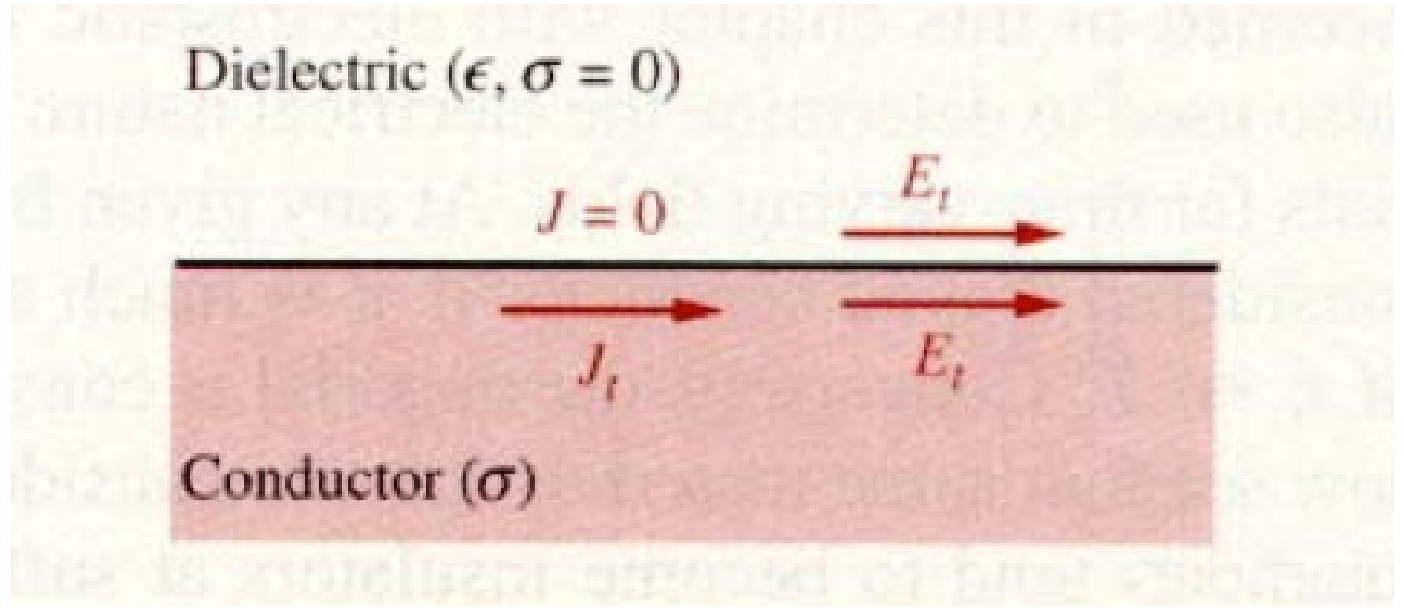
\includegraphics[scale=0.3]{elec-2}
\end{center}
En résumé : il y a à l'intérieur du conducteur une densité de courant $\vec{J}$ qui veut dire qu'il y a un champ $\vec{E}$ qui y règne et qui y est parallèle: $\vec{E}_{\text{int}} = \rouge{E_t} \vec{1}t$. Or en dehors du conducteur, on a une \bleu{composante normale au champ électrique}, tandis que \rouge{la composante tangentielle reste la même} !

\eq{\vec{E}_{\text{out}} = \rouge{E_t} \vec{1}_t + \bleu{E_n} \vec{1}_n}
La composante normale au champ électrique est due au fait que pour produire le champ adéquat dans le conducteur, des \textbf{charges de surface} se disposent d'une certaine manière, créant une composante normale au champ, qui \textbf{correspond à cette densité superficielle de charges sur le conducteur}.
\section{Aspects microscopiques : courant de conduction}
On s'intéresse à la nature du courant et aux phénomènes sous-jacents expliquant la conductivité d'un matériau.
\subsection{Courant de conduction $><$ courant de convection}
\begin{itemize}
\item Le courant de convection correspond au déplacement réel de matière chargée.
\item Le courant de conduction est dû au mouvement relatif des porteurs de charges libres à l'intérieur d'un conducteur. \textbf{Seul lui répond à la loi d'Ohm}.
\end{itemize}
\subsection{Vitesse des charges = vitesse de dérive}
\subsubsection{En l'absence champ extérieur}
Il faut savoir que même sans champ extérieur, les électrons sont en mouvement dans le conducteur, à très haute vitesse. Celle-ci est appelée \textit{vitesse thermique} $\vec{v}_h$, mais comme le mouvement est dans des orientations tout à fait aléatoire, le courant  résultant est nul.
\subsubsection{En présence d'un champ extérieur}
En présence d'un champ, les électrons sont accélérés : $\vec{F} = q\vec{E} = m\vec{a}$ donc sur une durée $\Delta t = t_c$ entre deux collisions ils acquièrent une vitesse $\vec{v}_d = \dfrac{q_e}{m} t_c \vec{E}$. Il s'agit de la vitesse d'ensemble des électrons, appelée \textbf{vitesse de dérive}.
\section{Puissance dissipée : effet Joule}
\bfe{6}{0.3}{\vspace{-1cm} \begin{eqnarray*}
p &=& \varrho \vec{E} \cdot \vec{v} \\
\vec{J} &\equiv& \varrho \vec{v} \\
p &=& \vec{J}\cdot \vec{E} \\
P_J &=& \int_\tau \vec{J}\cdot \vec{E} d\tau
\end{eqnarray*}}
Une certaine quantité de charge (volum $\tau$ densité $\varrho$) en mouvement à vitesse $\vec{v}$ soumise à un champ électrique et donc à une force par quantité de volume $\vec{f} = \varrho \vec{E}$ va se déplacer suite à cette force, et on peut calculer la puissance développée par $\vec{f}$, et ensuite l'intégrer sur $\tau$ pour trouver la puissance totale développée. \\

On peut obtenir la puissance développée d'une autre manière en réalisant un bilan d'énergie comme fait dans le cours PHYS-H1002. $$dW = V \ dQ \iff P = IV$$

\section{Équations de Maxwell et loi des noeuds}
Conducteur entouré d'un matériau isolant, et on part de l'équation de continuité :

\eq{ \oint_S \vec{J}.d\vec{S} + \dfrac{d\varrho}{dt} = 0}

L'intégrale de flux sur une surface fermée qui englobe plusieurs fils se décompose en : 
\begin{enumerate}
\item La somme algébrique des courants (parce que l'intégrale de flux fait intervenir un produit scalaire, le sens compte).
\item Le flux du courant sur la surface isolante, qui lui est nul, par définition de la surface isolante.
\end{enumerate}
Enfin, comme dans un conducteur on considère qu'on a une \textbf{densité volumique de charge nulle}, on a :

\eq{\sum_j I_j = 0}
\section{Loi des mailles et force électromotrice}
\subsection{Justification de la loi des mailles}
Si la circulation du courant dissipe de l'énergie, c'est que celle-ci provient d'une source : le générateur qui transforme de l'énergie non-électrique en énergie électrique.
\subsubsection{Loi des mailles}
La circulation du champ électrique sur tout contour fermé est nulle. Or le champ électrique peut être défini par un potentiel, donc la somme des variations de potentiel le long de toute maille \textbf{fermée} est nulle !

\eq{\oint_C \vec{E}.d\vec{l} = 0 \iff \sum_{\text{circuit}} \Delta V_i = 0}

\subsection{Rôle du générateur dans un circuit}
Si le générateur arrive à faire circuler les charges du + vers le -, c'est qu'à l'intérieur celles-ci voyagent du - vers le +. Ceci n'est pas un problème parce que le générateur transforme justement une énergie \textbf{extérieure, ne répondant pas aux équations de Maxwell} en une énergie électrique qui elle, doit répondre aux équations de Maxwell.
\subsection{Modélisation : force électromotrice}
Notons $\vec{f}_s$ la force par unité de charge qui provoque le mouvement des charges positives du - vers le +. Dans le générateur, on a donc une force totale $\vec{f}_{tot}$, la \textbf{force nette par unité de charge}, telle que reprise ci-dessous : en effet, le champ électrique est là sur tout le chemin !

\eq{\vec{f}_{tot} = \vec{f}_s + \vec{E}}
\subsubsection{Force électromotrice}
\bb{\underline{Définition} : la force électromotrice est la circulation de la force nette par unité de charge sur toute la longueur du circuit}
Mathématiquement : $$ \mathcal{E} = \oint_C \vec{f}_{tot} .d \vec{l} = \oint_C \vec{f}_{s} .d \vec{l} + \underbrace{\oint_C \vec{E} .d \vec{l}}_{=0} = \int_a ^b \vec{f}_s .d\vec{l}$$
La f.é.m peut être interprétée comme le \textbf{travail par unité de charge fourni par la source}.

\chapter{Magnétostatique dans le vide}
Dans ce chapitre on va faire \bleu{\textbf{comme pour l'électrostatique dans le vide}} mais pour la magnétostatique, c'est-à-dire \bleu{résoudre les équations de Maxwell associées}, \bleu{résoudre des problèmes de magnéto}, \bleu{introduire le \textbf{potentiel vecteur}}, \bleu{calculer un champ magnétique en tout point de l'espace} (\textbf{Biot-Savart}), \bleu{s'intéresser aux conditions limites s'appliquant à une surface parcourue par un courant}, et ensuite s'intéresser aux coefficients d'inductance, \bleu{parler de l'énergie magnétique}, de dipôle magnétique, les couples \& forces agissant sur un courant dans un champ magnétique, et finalement parler de l'effet Hall. 

\section{Équations de Maxwell}
Concernant le champ magnétique dans le vide et en statique, les équations de Maxwell utiles sont :

\begin{eqnarray*}
\div \vec{B} = 0 &\iff& \oint_S \vec{B}.d\vec{S} = 0 \qquad \forall S \\
\rot \vec{B} = \mu_0 \vec{J} &\iff& \oint _C\vec{B}.d\vec{l} = \mu_0 I \qquad \forall C
\end{eqnarray*}

Ici, le champ magnétique $\vec{B}$ représente l'effet de toutes les charges en muvement du problème. Il permet de calculer la force magnétique de Lorentz, et ainsi de compléter la force :

\eq{\vec{f}_m = q_0 (\vec{E} + \vec{v} \times \vec{B})}
La force fait ici intervenir un produit vectoriel, parce que contrairement à l'électrostatique, la cause de la force n'est plus là une simple charge $q_0$, mais un vecteur de déplacement $q_0 \vec{v}$, dont il faut prendre le sens en compte ! Dans l'expression de la force de Lorentz, on retrouve toutes les influences des autres charges susceptibles d'influencer $q_0$ : les charges fixes pour $\vec{E}$ et les charges mobiles pour $\vec{B}$.
\section{Champ magnétique}
Les propriétés principales du champ magnétique sont sa divergence nulle, sa circulation proportionnelle au courant qu'il embrasse, et qu'il \textbf{respecte le principe de superposition} (les équations de Maxwell sont linéaires).

\subsection{Champ magnétique du à un courant rectiligne}
\begin{eqnarray*}
\text{Intérieur } &:& \vec{B} = \dfrac{\mu_0}{2\pi r} \ I\ \vec{1}_\phi \qquad \text{circulation de $\vec{B}$ sur un cercle de rayon $r$} \\
\text{Extérieur } &:& \vec{B} = \dfrac{\mu_0}{2\pi} \dfrac{r}{b^2}\ I\ \vec{1}_\phi
\end{eqnarray*}
\subsection{Champ du à un solénoide}
\bfe{5}{0.3}{\vspace{-1cm}
\begin{eqnarray*}
\vec{B} &=& B(r) \vec{1}_z \\
\vec{B}_{ext} &=& \vec{0} \\
\vec{B}_{in} &=& \dfrac{\mu_0 N}{L}\ I\ \vec{1}_z
\end{eqnarray*}}
On suppose le solénoïde infini, donc le champ ne peut pas dépendre de $z$. Le champ ne peut pas non plus dépendre de $\phi$ par symétrie du cylindre, donc $\vec{B}$ ne dépend que de $r$. Les sources de $\vec{B}$ sont orientés selon  $\vec{1}_phi$, donc $\vec{B}$ n'a pas de composantes selon $\vec{1}_\phi$. De plus, $\vec{B}$ ne peut pas avoir de composante lamellaire donc pas de composante selon $\vec{1}_z$. Pour la quantification, il ne suffit que de prendre des intégrales de circulation pour s'assurer que le champ magnétique est nul à l'extérieur, et proportionnel au nombre de spires \& l'intensité de courant balayé.
\subsection{Champ du à un courant torique}
\wraparray{3}{0.2}{\vec{B}_{ext} &=& \vec{0} \\
\vec{B}_{in} &=& \dfrac{\mu_0 N I}{2\pi r} \vec{1}_\phi}
On effectue l'intégrale de circulation sur un contour circulaire de rayon $r$ englobant un courant $NI$ pour avoir le champ magnétique.

\section{Potentiel vecteur magnétique}
Comme la divergence du rotationnel est nulle tout comme celle du champ magnétique, c'est peut-être parce que le champ magnétique est lui-même le rotationnel d'un autre champ de vecteurs qu'on appelle \textbf{potentiel vecteur} $\vec{A}$. Celui-ci est défini à une constante près parce que le rotationnel fait intervenir des dérivées partielles (spatiales). On peut donc toujours ajoute un vecteur $\vec{f}$ à $\vec{A}$ pour autant que le rotationnel de $\vec{f}$ soit nul, donc que $\vec{f}$ dérive d'un potentiel qu'on notera $\varphi$. Donc si $\vec{A}$ est un potentiel vecteur satisfaisant un problème de magnéto, alors tout $\vec{A}'$ aussi tel que :

\eq{\vec{A}' = \vec{A} + \grad \varphi}

\subsubsection{Jauge de Coulomb}
Une \textbf{jauge} est une condition qu'on ajoute sur le potentiel pour avoir un point de référence. Ici, pour définir le champ scalaire additif $\varphi$, on imposera que $\div \vec{A}$ s'annule.

\subsection{Équation et formules du potentiel vecteur}
\wraparray{8}{0.4}{\Delta A_x &=& -\mu_0 J_x \\
\Delta V &=& -\dfrac{\varrho}{\varepsilon_0}  \Rightarrow V = \dfrac{1}{4\pi \varepsilon_0} \int_\tau \dfrac{\varrho}{R} d\tau \\
\Rightarrow A_x &=& \dfrac{\mu_0}{4\pi} \int_\tau \dfrac{J_x}{R} d\tau \\
\Rightarrow \vec{A} &=& \dfrac{\mu_0}{4\pi} \int_\tau \dfrac{\vec{J}}{R} d\tau}
Comme $\rot \vec{B} = \mu_0 I$, il faut que $\rot \rot \vec{A} = \mu_0 I$. Sauf que $\rot \rot \vec{A} = -\Delta \vec{A}$ vu que la divergence de $\vec{A}$ est nulle. On arrive alors à une équation qui ressemble à celle de Poisson pour le potentiel électrique (en prenant composante par composante). La clé est d'alors établir l'analogie avec le potentiel électrique pour la résolution de l'équation de Poisson. \\

Dans le cas d'un courant filiforme, $\vec{J} = I d\vec{l}$ et dans le cas d'une nappe de courant, on note la densité de courant de surface $\vec{K}$ et on intègre sur une surface $S$ :

\eq{\text{Nappe de courant : }\vec{A} = \dfrac{\mu_0}{4\pi} \int_S \dfrac{\vec{K}}{R} dS}
\subsection{Interprétation du potentiel vecteur}
\wraparray{6}{0.3}{\Phi &=& \int_S \vec{B}.d\vec{S} \\
&=& \int_S \rot \vec{A}.d\vec{S} \\
&=& \oint_C \vec{A}.d\vec{l}}
La circulation du potentiel vecteur magnétique sur un contour est égale au flux magnétique à travers une surface sous-tendue à ce contour.
\section{Formule de Biot-Savart}
Pas de démonstration :

\bo{\eq{\text{Biot-Savart : }  \vec{B} = \dfrac{\mu_0}{4\pi} \int_{\tau'} \dfrac{\vec{J} \times \vec{1}_r}{R^2} d\tau'}}
\section{Conditions aux limites}
\subsection{Variation du champ $\vec{B}$}
On va démontrer dans cette section que lors d'un passage au travers une surface caractérisée par une densité de courant de surface $\vec{K}$, le champ magnétique est \textbf{discontinu} :

\eq{\vec{1}_n \times (\vec{B}_1 - \vec{B-2}) = \mu_0 \vec{K}}
\subsubsection{Composante normale}
La divergence de $\vec{B}$ est nulle, donc la composante normale est continue.
\subsubsection{Composante tangentielle}
\wraparray{5}{0.3}{
(B_1 - B_2) L &=& \mu_0 KL \\
(B_1 - B_2)_t &=& \mu_0 K \\
\vec{1}_n \times \Vert \vec{B} \Vert &=& \mu_0 \vec{K}}
Quand on prend la circulation du champ $\vec{B}$ sur un contour qui traverse la surface, on obtient que la différence des composantes tangentielle est proportionnelle à la densité de courant de surface.
\section{Coefficients d'inductance}
On sait que $\vec{A}_1 \propto I_1$. Par ailleurs, le flux embrassé par un contour 2 $\Phi_{21} \propto \vec{A}_1 \propto I_1$. Cela nous amène à définir un coefficient dit d'\q{inductance}, noté $L_{21}$ qui caractérise l'influence du circuit 1 sur le circuit 2.

\eq{\Phi_{21} = L_{21} I_1}

La définition du coefficient d'inductance  est ici, c'est le rapport du flux sur le courant qui cause ce flux. En notant $\Psi = N_2 \Phi$ si on met $N_2$ spires dans le circuit 2 :

\eq{L_{21} = \dfrac{\Psi_{21}}{I_1} = \dfrac{N_2}{I_1} \oint_{C_2} \vec{A_1}.d\vec{l}_2}

Or pour des courants filiformes (un circuit fermé disons), il existe une relation entre $I_1$ et $\vec{A}_1$ ! La relation était la suivante :

\eq{\vec{A}_1 = \dfrac{\mu_0}{4\pi} \oint_{C_1} \dfrac{I_1}{R} d\vec{l}_1}
On peut donc affiner la formule du coefficient d'inductance :

\eq{L_{ij} = \dfrac{\mu_0 N_iN_j}{4\pi} \oint_{C_j} \oint_{C_i} \dfrac{d\vec{l}_i . d\vec{l}_j}{R}}

\section{Énergie magnétique}
On associe à toute distribution de courant une énergie magnétique, qui est à interpréter comme le travail nécessaire pour mettre en mouvement les charges qui ont permis de constituer ces courants.
\subsection{Énergie magnétique associée à un courant et densité d'énergie magnétique}
Par de simples analogies :
\begin{eqnarray*}
W_e = \dfrac{1}{2} \int_\tau \varrho V d\tau \qquad &\Rightarrow& \qquad W_m = \dfrac{1}{2} \int_\tau \vec{J}.\vec{A} d\tau \\
w_e = \dfrac{1}{2} \varepsilon_0 E^2 \qquad &\Rightarrow & \qquad w_m = \dfrac{1}{2\mu_0} B^2
\end{eqnarray*}
\subsection{Énergie associée à un ensemble de courants}
Considérons un ensemble de volumes $D_i$ avec $i$ allant jusqu'à $n$, chacun parcouru par un courant constant $I_i$ de densité $\vec{J}_i$. Alors, l'énergie magnétique associée à cet ensemble de courants vaut :
$$W_m = \dfrac{1}{2} \sum_i \sum_j \int_{Di} \vec{J}_i.\vec{A}_j d\tau$$
\subsection{Énergie magnétique exprimée en fonction des coefficients d'inductance}
Compte tenu de la définition des coefficients d'inductance, l'énergie totale d'un système de courants peut s'écrire comme : $$W_m = \dfrac{1}{2} \sum_i \sum_j L_{ij} I_i I_j $$
Ou, pour un circuit filiforme fermé unique : $$W_m = \dfrac{1}{2}LI^2$$
On remarque qu'on peut déduire le coefficient d'inductance à partir de l'énergie magnétique d'un système.

\section{Dipôle magnétique}
Très brièvement, un dipôle magnétique est une boucle filiforme parcourue par un courant $I$.
\subsection{Moment dipolaire $\vec{m}$}
Pour une boucle circulaire, \textbf{la définition du moment dipolaire }est : $$\vec{m} = IS\vec{1}_n$$

\subsection{Potentiel et champ autour du dipôle}
Tout comme on pouvait calculer le potentiel électrique généré par un dipôle électrique ($V = \dfrac{1}{4\pi\varepsilon_0} (\vec{p}\cdot \vec{1}_R)/R^2$), on a ici : $$\vec{A} = \dfrac{\mu_0}{4\pi} \dfrac{\vec{m} \times \vec{1}_R}{R^2} $$

\section{Forces et couples sur des courants}
\subsection{Sur un élément de courant}
\wraparray{6}{0.3}{
\vec{F} &=& q_e \vec{v} \times \vec{B} \\
d\vec{F} &=& \varrho \vec{v} \times \vec{B} d\tau \\
&=& \vec{J} \times \vec{B} A \ dl \\
&=& I \ d\vec{l} \times \vec{B} \\
}
Sur une quantité de charge $q_e$ en mouvement, la force exercée est $\vec{F}$ : il s'agit de la force magnétique de Lorentz. Si l'on considère un fil parcouru par un courant, et qu'on prend un élément de volume $d\tau$ de ce fil, la force exercée est celle exercée sur un élément de charge $q_e N_e d\tau$, avec $N_e$ le nombre de charges dans ce volume, donc $q_e N_e = \varrho_e$. Ceci nous fournit une expression dans laquelle on voit apparaître en produit $\vec{v}_e$ et $\varrho_e$ qui n'est rien autre que $\vec{J}$. La densité de courant est égale à l'intensité divisée par la section $A$ du fil, qui se simplifiera avec le $A$ contenu dans l'élément de volume.
\subsection{Sur un circuit fermé}
\wraparray{2}{0.3}{\vec{F} &=& \oint_C I \ d\vec{l} \times \vec{B} = 0}
Il faut intégrer la force sur un élément de courant sur tout un contour fermé mais on obtiendra 0 parce que le courant est identique sur toute section du fil. On interprète en disant que sur un circuit fermé, les forces agissant sur les parties du circuit s'annulent les unes les autres.
\subsection{Sur un cadre rectangulaire dans $\vec{B}$ uniforme}
Il y aura deux côtés sur lesquels les forces vont se compenser, et deux côtés où les forces seront opposées et pas sur le même support : il y aura donc un moment de force. La force aura en module $$F = I \cdot b \cdot B,$$
et le couple de forces résultant est 
$$\vec{C} = a\sin \theta F \vec{1}_x = I \cdot ab \cdot B\sin\theta \vec{1}_x = \vec{m}\times \vec{B}.$$

Cette brève étude permet de voir qu'une boucle parcourue dans un courant subit un couple de forces lorsque plongée dans un champ magnétique. Celui-ci restera non nul tant que la boucle ne s'est pas orientée perpendiculairement au champ (tant que le vecteur normal de surface n'est pas parallèle à $\vec{B}$).

\bo{Couple : $\vec{C} = \vec{m} \times \vec{B}$}

\section{Effet Hall}
Lire le sylla est super intéressant. L'effet Hall est observé dans un conducteur/semi-conducteur parcouru par un courant et plongé dans un champ magnétique \textbf{externe}. Il en résulte une différence de potentiel, par séparation des charges parce que les charges positives et négatives subissent le champ magnétique de deux manières opposées. Lorsque les charges sont séparées, il y a une différence de potentiel entre elles ce qui va engendrer un champ électrique entre les deux plaques supérieure et inférieure du trucmuche. Le champ électrique va engendrer une force sur ces charges, qui est de nature opposée à la force magnétique ! \\

En régime stationnaire, on a une situation d'équilibre. Une petite interprétation permet de lever un point intéressant :

\begin{itemize}
\item On vient de voir qu'un champ magnétique provoquait pour les charges en mouvement, une séparation des charges et donc une force d'origine électrostatique.

\item Cela veut dire que si l'on prend un fil parcouru de courant et qu'on le plonge dans un champ magnétique, il va se passer pareil ! La force $F = I \vec{L}\times \vec{B}$ est en réalité d'origine électrostatique par polarisation des charges à cause du champ magnétique.
\end{itemize}

\chapter{Milieux magnétiques}
Tout comme en électrostatique dans les milieux diélectriques, on constate qu'en présence de certains matériaux, les résultats obtenus ne sont pas cohérent avec la matière étudiée au chapitre précédent. Se posent la question de \q{comment modifier les équations de Maxwell}, \q{comment expliquer ces nouveaux phénomènes}, et \q{comment sont modifiés les résultats obtenus}. Les matériaux ici étudiés sont les matériaux dits \textbf{magnétiques}.
\section{Comment étendre les équations de Maxwell aux milieux magnétiques ?}
On constate premièrement que le champ total relevé, $\vec{B}$, ne correspond pas au champ généré par les courants libres $\vec{J}$. Plus précisément : on remarque que si on calcule le champ $\vec{B}$ par $\rot \vec{B} = \mu_0 \vec{J}$ et qu'on l'injecte dans $\vec{F} = q_0\vec{v}\times\vec{B}$, on n'obtient pas la force réelle mesurée. \\

Alors comme en électrostatique, on dit qu'en réalité il y a une partie du champ qui est due aux courants libres, et une autre due à des courants dits de magnétisation. Alors la loi d'Ampère est valable si dans $\vec{B}$ se trouve $\vec{B}_l + \vec{B}_m$ et dans  $\vec{J}$ se trouve $\vec{J}_l + \vec{J}_m$. De manière intégrale on a alors $I = I_l + I_m$.

\section{Matériaux magnétiques et magnétisation}
\subsection{Hypothèse}
Pour justifier la présence de $\vec{J}_m$ ($I_m$), on fait l'hypothèse que dans un matériau magnétique se crée un champ magnétique $\vec{B}_m$, généré par des dipoles magnétiques. Pour  rappel : à chaque dipole on associe un moment dipolaire $\vec{m} = IS \vec{1}_n$.

\subsection{Champ $\vec{M}$ : magnétisation}
Le champ $\vec{M}$ est une densité volumique de dipoles magnétiques. Il modélise le phénomène de magnétisation.
\eq{\vec{m} = \int_\tau \vec{M}d\tau}
\subsection{Potentiel vecteur et champ générés par de la matière magnétisée}
\wraparray{3}{0.3}{&\text{Volume : }&\vec{J}_m = \rot \vec{M} \\ &\text{Surface : }&\vec{K}_m = \vec{M} \times \vec{1}_n}
On vient de voir qu'un matériau magnétique avait une densité non nulle de moments dipolaires. Ceux-ci génèrent  donc un champ, et donc on peut les associer à un potentiel ! Tout ça est lié à $\vec{M}$. En particulier : les \textbf{courants de magnétisation} dont la densité volumique est notée $\vec{J}_m$ et la densité surfacique est notée $\vec{K}_m$. Le potentiel vecteur associé quant à lui vaut :

\eq{\vec{A}_m \quad =  \quad\dfrac{\mu_0}{4\pi} \int_V \dfrac{\vec{J}_m}{R} d\tau \quad +\quad \dfrac{\mu_0}{4\pi} \oint_S \dfrac{\vec{K}_m}{R} dS}
Dont on peut tranquillement prendre le rotationnel pour calculer le champ magnétique engendré par la magnétisation,  $\vec{B}_m = \rot \vec{A}_m$.
\section{Champ magnétisant $\vec{H}$ et relation constitutive}
\wraparray{11}{0.4}{\rot \vec{B} &=& \mu_0(\vec{J}_l + \rot \vec{M}) \\ \vec{J_l} &=& \rot \left(\bleu{ \dfrac{1}{\mu_0} \vec{B} - \vec{M}} \right) \\
\vec{H} &=& \bleu{\dfrac{1}{\mu_0} \vec{B} - \vec{M}} \\
\vec{D} &=& \varepsilon_0 \vec{E} + \vec{P} \\
\rot \vec{H} &=&  \vec{J}_l \\
\oint_C \vec{H}.d\vec{l} &=&  I_l \
}
Comme on arrive à écrire $\vec{J}_m = \rot \vec{M}$, on peut écrire que $\vec{J}_l$ est le rotationnel d'un champ qu'on nommera \textbf{champ magnétisant} $\vec{H}$ qui est donc un champ magnétique exclusivement du aux courant libres de densité $\vec{J}_l$. L'intégrale de circulation de ce champ sur un contour fermé donne donc les \textbf{courants libres} enfermés par ce contour. On voit clairement cette fois qu'en magnétostatique, l'équivalent de $\varepsilon_0$ c'est $\frac{1}{\mu_0}$, e on voit que l'équivalent de $\vec{D}$ c'est $\vec{H}$, l'équivalent de $\vec{P}$ c'est $-\vec{M}$.

\subsection*{Interprétation}
Le champ $\vec{H}$ est du aux courants libres, il s'agit donc d'un \q{champ source}. Le champ magnétique total qu'on peut relever est $\vec{B}$ et est un \q{champ effet} parce qu'il tient compte des effets de magnétisation. Le champ $\vec{M}$ représente quant à lui l'impact de la magnétisation.

\bo{Relation constitutive : $\vec{H}=\dfrac{1}{\mu_0} \vec{B} - \vec{M}$}
La notion de force magnétomotrice désigne le courant qui enroule un matériau magnétique, le courant responsable du phénomène de magnétisation. Supposons qu'on enroule un fil traversé par un courant $I$ qu'on enroule $N$ fois sur un matériau magnétique.

\eq{\mathcal{F} = \oint \vec{H}.d\vec{l} = I_l = NI}
Les unités sont des ampères-tours ($At$) et correspond au nombre de tours réalisés avec un fil supportant un certain nombre d'ampères.

\section{Milieux magnétiques linéaires}
\subsection{Matériaux magnétiques linéaires}
\wraparray{6}{0.3}{
\vec{B} &=& \mu \vec{H} \iff \vec{M} \propto \vec{H} \\
\vec{M} &=& \chi_m \vec{H} \\
\Rightarrow\vec{B}&=& \mu_0 (1+\chi_m)\vec{H} \\
\Rightarrow \mu &=& \mu_0(1+\chi_m)
}
Dans le vide, $\vec{H}$ est lié à $\vec{B}$ de la simple constante $\mu_0$. Dans un matériau magnétique, la constante est la perméabilité du milieu. Si elle est constante, le matériau est magnétique linéaire.  On peut quantifier $\mu$ comme on l'a fait en électrostatique. Notons que la perméabilité relative $\mu_r$ vaut $(1+\chi_m)$. \\

Le matériau est dit \q{homogène} si sa perméabilité est constante dans l'espace. La densité de courants de magnétisation est alors proportionnelle à la densité de courants libres : $$\vec{J}_m = \rot \vec{M} = \rot (\chi_m \vec{H}) = (\mu_r-1) \vec{J}_l$$
Ainsi, la densité de courant \textbf{totale} vaut $\mu_r \vec{J}_l$, et la loi d'Ampère se réécrit :
$$\rot \vec{B} = \mu_0 \vec{J} = \mu \vec{J}_l$$.

\section{Origine physique de la magnétisation (interprétation des courants de magnétisation)}
\subsection{Para- et diamagnétisme}
C'est super simple. Dans les matériaux il y a des électrons en mouvement, en rotation, en orbite, pour plusieurs raisons, et c'est ce mouvement qui cause des courants microscopiques et donc les phénomènes magnétiques. Ces mouvements sont le spin de l'électron et l'orbite de l'électron autour du noyau. Chaque courant atomique correspond à un dipôle magnétique auquel on associe un moment dipolaire et donc un champ magnétique. \\

Sans champ extérieur, les moments dipolaires orbitaux s'annulent en moyenne, tandis que les spins peuvent donner un $\vec{m}\neq\vec{0}$. \\

\begin{description}[leftmargin=!,labelwidth=\widthof{\bfseries PParamagnétisme}]
\item[Paramagnétisme] Moments dipolaires permanents qui sont renforcés par l'apparition d'un $\vec{B}$ extérieur (moments vont s'orienter vers $\vec{B}$.
\item[Diamagnétisme] Moments dipolaire nul initialement. Le champ magnétique vient tout chambouler, alors par loi de Lenz (conservation de l'énergie), la variation de moment dipolaire est dirigée dans le sens opposé au champ externe.
\end{description}
Ces deux phénomènes sont cependant très peu significatifs.
\subsection{Lien avec le vecteur de magnétisation $\vec{M}$}
Sous l'effet d'un champ magnétique, on vient de voir que les dipôles magnétiques prennent une certaine orientation. Selon si le matériau est paramagnétique ou diamagnétique, le moment dipolaire va contribuer ou s'opposer au champ magnétique. Il y a donc véritablement une \textbf{densité de moment dipolaire moyen non nulle} : c'est l'interprétation du vecteur $\vec{M}$.

\section{Conditions aux limites}
On va s'intéresser aux composantes du champ source lorsqu'il traverse une surface qui délimite deux milieux de perméabilité différente.
\subsection{Composante normale}
On sait que la composante normale du champ effet $\vec{B}$ est continue. Alors par la relation constitutive, on a :$$H_{1n}-H_{2n} = -(M_{1n}-M_{2n}).$$
Par ailleurs, si les deux milieux sont des matériaux linéaires :
$$\mu_1H_{1n}=\mu_2H_{2n}$$
\subsection{Composante tangentielle}
On peut appliquer l'intégrale de circulation sur $\vec{H}$ sur un contour fermé qui passe par la surface. Si la surface est parcourue par un courant de densité surfacique $\vec{K}_l$, alors :

$$\vec{1}_n \times (\vec{H}_1 - \vec{H}_2) = \vec{K}_l.$$ Ceci veut précisément dire que la composante tangentielle est continue en l'absence de courant sur la surface ($\vec{K}_l = \vec{0}$). Pour le champ magnétique effet, on a :
\begin{eqnarray*}
B_{1n} &=& B_{2n} \\
\dfrac{B_{1t}}{\mu_1} &=& \dfrac{B_{2t}}{\mu_2}
\end{eqnarray*}
\section{Le ferromagnétisme}
C'est super super cool.
\chapter{Quasi-statique : induction magnétique}
\end{document}